\documentclass{article}

\usepackage{tikz}
\usetikzlibrary{decorations}
\usetikzlibrary{calc}
\usetikzlibrary{decorations.pathreplacing}
\usepackage{amsmath}
\usepackage{hyperref,cleveref}
\usepackage{mathtools}

\DeclarePairedDelimiter\ceil{\lceil}{\rceil}
\DeclarePairedDelimiter\floor{\lfloor}{\rfloor}

\title{Algoritmo per schede di palestra vincolate}

\begin{document}

\section{Problema}
Il problema nasce dalla necessità di una strategia veloce e corretta per la
creazione di una scheda di palestra che rispetti determinati vincoli fisici.
L'obiettivo è quello di fornire un algoritmo che riesca a rielaboare velocemente
una scheda in seguito alla modifica di uno qualsiasi dei parametri di essa.
I vincoli da rispettare sono:
\begin{itemize}
    \item Il numero di giorni di allenamento alla settimana, adattato
    all'esigenza dell'utente
    \item Per ogni giorno, il numero massimo di serie, oltre il quale l'energia
    posseduta dal corpo non è più sufficiente per una esecuzione efficace di un
    qualsiasi esercizio
    \item Per ogni muscolo, il numero massimo di serie giornaliere, oltre il
    quale il muscolo non è più in grado di rispondere in maniera ottimale
    \item Per ogni muscolo, il numero minimo di serie settimanali, senza le
    quali il muscolo non cresce in maniera ottimale
\end{itemize}

\section{Formalizzazione}

Dati $N$ giorni $g_1, g_2, ..., g_N$, dove ogni giorno ha un massimo di serie
giornaliere pari a $maxg$ e $M$ muscoli $m_1, m_2, ..., m_M$, dove ogni muscolo
ha un massimo di serie giornaliere $max_1, max_2, ..., max_M$ e un minimo di
serie settimanali $min_1, min_2, ..., min_M$. L'algoritmo deve ritornare un
insieme $S$ di assegnazioni giorno, muscolo, serie $(g, m, s)$ tale che valga:

\begin{enumerate}
    \item \label{one}   $g \leq N$, $m \leq M$
    \item \label{two}   $\forall i \in \{1...N\} \sum_{s \in \{S | g = i\}}s \leq maxg$ (per ogni giorno il numero di serie deve essere inferiore al massimo giornaliero)
    \item \label{three} $\forall i \in \{1...M\} \sum_{s \in \{ S | m = i\}} s \geq min_i$ (per ogni muscolo il numero di serie settimanali deve essere almeno pari al minimo settimanale)
    \item \label{four}  $\forall i \in \{1...N\}, j \in \{1...M\} \sum_{s \in \{S | g = i, m = j\}} s \leq max_i$ (per ogni giorno, ogni muscolo non può superare il suo massimo giornaliero)
\end{enumerate}

\section{Implementazione}
L'algoritmo fa utilizzo della tecnica di Ford-Fulkerson per la ricerca del
flusso massimo.
Viene creato un grafo del seguente tipo:

\begin{center}
    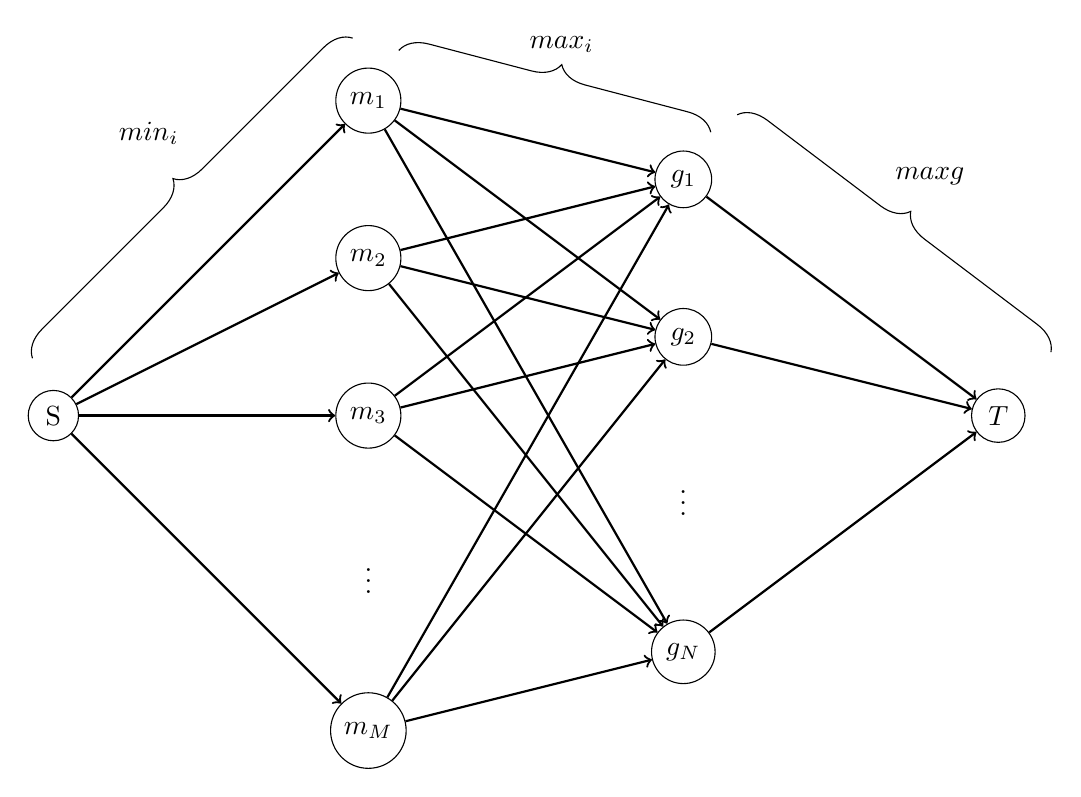
\begin{tikzpicture}
        \node[draw, circle] (S)     at (0,0)    {S};
        \node[draw, circle] (m1)    at (4,4)    {$m_1$};
        \node[draw, circle] (m2)    at (4,2)    {$m_2$};
        \node[draw, circle] (m3)    at (4,0)    {$m_3$};
        \node[draw=none]    (mdots) at (4,-2)   {$\vdots$};
        \node[draw, circle] (mm)    at (4,-4)  {$m_M$};

        \draw [decorate,decoration={brace,amplitude=10pt,raise=20pt}] (S.north east) -- (m1.north east) node[midway,above,yshift=30pt,xshift=-30pt] {$min_i$};
        \draw[->][thick] (S) -- (m1);
        \draw[->][thick] (S) -- (m2);
        \draw[->][thick] (S) -- (m3);
        \draw[->][thick] (S) -- (mm);

        \node[draw, circle] (g1)    at (8,3)    {$g_1$};
        \node[draw, circle] (g2)    at (8,1)    {$g_2$};
        \node[draw=none]    (gdots) at (8,-1)   {$\vdots$};
        \node[draw, circle] (gn)    at (8,-3)   {$g_N$};

        \draw [decorate,decoration={brace,amplitude=10pt,raise=10pt}] (m1.north east) -- (g1.north east) node[midway,above,yshift=20pt,xshift=5pt] {$max_i$};
        \draw[->][thick] (m1) -- (g1);
        \draw[->][thick] (m1) -- (g2);
        \draw[->][thick] (m1) -- (gn);
        \draw[->][thick] (m2) -- (g1);
        \draw[->][thick] (m2) -- (g2);
        \draw[->][thick] (m2) -- (gn);
        \draw[->][thick] (m3) -- (g1);
        \draw[->][thick] (m3) -- (g2);
        \draw[->][thick] (m3) -- (gn);
        \draw[->][thick] (mm) -- (g1);
        \draw[->][thick] (mm) -- (g2);
        \draw[->][thick] (mm) -- (gn);

        \node[draw, circle] (T) at (12,0) {$T$};

        \draw [decorate,decoration={brace,amplitude=10pt,raise=20pt}] (g1.north east) -- (T.north east) node[midway,above,yshift=30pt,xshift=25pt] {$maxg$};
        \draw[->][thick] (g1) -- (T);
        \draw[->][thick] (g2) -- (T);
        \draw[->][thick] (gn) -- (T);

    \end{tikzpicture}
\end{center}

Il costo computazionale per la creazione del grafo è $O(MN)$.
È possibile automatizzare la scelta di $maxg$ in modo da uniformare il numero di
serie giornaliere, questo viene fatto assegnando a $maxg$ il valore atteso del
numero di serie giornaliere $\ceil{\sum_{i=1}^Mmin_i / N}$ con costo
$O(M)$.
Successivamente viene applicato l'algoritmo di Ford-Fulkerson.
\begin{itemize}
    \item Il vincolo \ref{one} è garantito dalla definizione del problema
    \item Per la verifica del vincolo \ref{two} gli archi
    $(g_j, T) \; \forall j \in 1...N$ hanno capacità pari a $maxg$
    \item Il vincolo \ref{three} invece deve essere verificato manualmente,
    controllando che valga $w(S, m_i) \geq min_i \; \forall i \in 0...M$ in
    tempo $O(M)$.
    \item Il vincolo \ref{four} è verificato dal fatto che gli archi
    $(m_i, g_j) \; \forall i \in 0...M, j \in 0...N$ hanno capacità pari a
    $max_i$
\end{itemize}
Infine vengono presi gli archi di tipo $(m_i, g_j)$ con flusso positivo, che
corrisponderanno alle assegnazioni. Le assegnazioni vengono poi ordinate per
giorno in tempo $O((NM) \log NM)$.
Ricapitolando gli step dell'algoritmo sono:
\begin{itemize}
    \item Creazione del grafo $O(MN)$
    \item Calcolo di $maxg$ $O(M)$
    \item Applicazione algoritmo di Ford-Fulkerson $O((M + N)^2 |f^*|)$
    \item Verifica di $w(S, m_i) \geq min_i \; \forall i \in 0...M$ $O(M)$
    \item Ricerca assegnazioni $O(MN)$
    \item Ordinamento assegnazioni $O((MN) \log (MN))$
\end{itemize}
L'algoritmo finale ha costo complessivo pari alla somma dei precedenti:

\begin{equation*}
\begin{split}
    T(M, N) &= O((MN) + (M) + ((M+N)^2 |f^*|) + (M) + (MN) + (MN) \log (MN)) \\
            &= \boxed{O((M+N)^2 |f^*| + (MN) \log (MN))} \\
\end{split}
\end{equation*}

\section{Post-processing}
Al termine dell'algoritmo ci troviamo con una collezione di record (giorno,
muscolo, serie), ognuno di questi record può essere suddiviso in più
esercizi. Dati i valori $K$ numero di serie del record e $mins$ e $maxs$
rispettivamente il numero minimo e massimo di serie per esercizio, dobbiamo
trovare un insieme $S$ tale che:
\begin{itemize}
    \item $\sum_{s \in S} s = K$
    \item $mins \leq s_i \leq maxs \; \forall s \in S$
    \item $|S|$ sia il più piccolo posssibile
    \item Il valore di $d = \sum_{s_1, s_2 \in S} |s_1 - s_2|$ sia il più
          piccolo possibile (la differenza tra il numero di serie tra due
          esercizi sia minimizzata)
\end{itemize}
Per fare ciò possiamo applicare il seguente algoritmo greedy:
\begin{itemize}
    \item Poniamo $|S| = \ceil{\frac{K}{maxs}}$ con ogni elemento di $S$
          pari a $maxs$
    \item Prendiamo un $s \in S$ diminuiamo $s$ di uno fino a quando
          $\sum_{s \in S} s$ diventa $K$ oppure fino a quando $s$ diventa $mins$
    \item Se alla fine dell'algoritmo $\sum_{s \in S} \neq K$ non esiste una
          soluzione e ritorniamo $\{ K \}$
    \item L'ultimo passo è quello di minimizzare la differenza tra i vari
          $s \in S$ per fare ciò poniamo $s_1 = \floor{(s_1 + s_1) / 2}$
          e $s_2 = \ceil{(s_1 + s_1) / 2} \; \forall s_1, s_2 \in S$.
\end{itemize}
L'algoritmo ha complessità
$O(MN * (maxs - mins) * \ceil{K / maxs} + \ceil{K / maxs}^2)$.
Supponendo che $mins$ e $maxs$ non facciano parte dell'input la complessità
diventa $O(MNK + K^2)$.

\section{Dimostrazione proprietà di scelta greedy (TODO)}

\end{document}
